% !TEX TS-program = XeLaTeX
% use the following command:
% all document files must be coded in UTF-8
\documentclass[portuguese]{textolivre}
% build HTML with: make4ht -e build.lua -c textolivre.cfg -x -u article "fn-in,svg,pic-align"

\journalname{Texto Livre}
\thevolume{19}
%\thenumber{1} % old template
\theyear{2026}
\receiveddate{\DTMdisplaydate{2026}{1}{29}{-1}} % YYYY MM DD
\accepteddate{\DTMdisplaydate{2026}{3}{18}{-1}}
\publisheddate{\DTMdisplaydate{2026}{9}{30}{-1}}
\corrauthor{Saulo Rogério Pacheco Rocha}
\articledoi{10.1590/1983-3652.2026.64127}
%\articleid{NNNN} % if the article ID is not the last 5 numbers of its DOI, provide it using \articleid{} commmand 
% list of available sesscions in the journal: articles, dossier, reports, essays, reviews, interviews, editorial
\articlesessionname{articles}
\runningauthor{Pacheco Rocha} 
%\editorname{Leonardo Araújo} % old template
\sectioneditorname{Daniervelin Pereira~\orcid{0000-0003-1861-3609}}
\layouteditorname{Rayany Chaves~\orcid{0009-0007-0028-484X}}

\title{O modelo de \textit{OCR Early Portuguese Printing no Transkribus}: sobre as inovações na transcrição de impressos históricos e os desafios da infraestrutura de pesquisa em linguística histórica e paleografia digital no Brasil}
\othertitle{The Early Portuguese Printing OCR Model in \textit{Transkribus}: on innovations in the transcription of historical printed documents and the research infrastructure for historical linguistics and digital paleography in Brazil}
% if there is a third language title, add here:
%\othertitle{Artikelvorlage zur Einreichung beim Texto Livre Journal}

\author[1]{Saulo Rogério Pacheco Rocha~\orcid{0000-0003-3715-6706}\thanks{Email: \href{mailto:saulorrp@gmail.com}{saulorrp@gmail.com}}}
\affil[1]{Universidade Federal de Santa Catarina, Centro de Comunicação e Expressão, Programa de Pós-Graduação em Linguística, Florianópolis, SC, Brasil.}

\addbibresource{article.bib}
% use biber instead of bibtex
% $ biber article

% used to create dummy text for the template file
\definecolor{dark-gray}{gray}{0.35} % color used to display dummy texts
\usepackage{lipsum}
\SetLipsumParListSurrounders{\colorlet{oldcolor}{.}\color{dark-gray}}{\color{oldcolor}}

% used here only to provide the XeLaTeX and BibTeX logos
\usepackage{hologo}

% if you use multirows in a table, include the multirow package
\usepackage{multirow}

% provides sidewaysfigure environment
\usepackage{rotating}

% CUSTOM EPIGRAPH - BEGIN 
%%% https://tex.stackexchange.com/questions/193178/specific-epigraph-style
\usepackage{epigraph}
\renewcommand\textflush{flushright}
\makeatletter
\newlength\epitextskip
\pretocmd{\@epitext}{\em}{}{}
\apptocmd{\@epitext}{\em}{}{}
\patchcmd{\epigraph}{\@epitext{#1}\\}{\@epitext{#1}\\[\epitextskip]}{}{}
\makeatother
\setlength\epigraphrule{0pt}
\setlength\epitextskip{0.5ex}
\setlength\epigraphwidth{.7\textwidth}
% CUSTOM EPIGRAPH - END

% to use IPA symbols in unicode add
%\usepackage{fontspec}
%\newfontfamily\ipafont{CMU Serif}
%\newcommand{\ipa}[1]{{\ipafont #1}}
% and in the text you may use the \ipa{...} command passing the symbols in unicode

% LANGUAGE - BEGIN
% ARABIC
% for languages that use special fonts, you must provide the typeface that will be used
% \setotherlanguage{arabic}
% \newfontfamily\arabicfont[Script=Arabic]{Amiri}
% \newfontfamily\arabicfontsf[Script=Arabic]{Amiri}
% \newfontfamily\arabicfonttt[Script=Arabic]{Amiri}
%
% in the article, to add arabic text use: \textlang{arabic}{ ... }
%
% RUSSIAN
% for russian text we also need to define fonts with support for Cyrillic script
% \usepackage{fontspec}
% \setotherlanguage{russian}
% \newfontfamily\cyrillicfont{Times New Roman}
% \newfontfamily\cyrillicfontsf{Times New Roman}[Script=Cyrillic]
% \newfontfamily\cyrillicfonttt{Times New Roman}[Script=Cyrillic]
%
% in the text use \begin{russian} ... \end{russian}
% LANGUAGE - END

% EMOJIS - BEGIN
% to use emoticons in your manuscript
% https://stackoverflow.com/questions/190145/how-to-insert-emoticons-in-latex/57076064
% using font Symbola, which has full support
% the font may be downloaded at:
% https://dn-works.com/ufas/
% add to preamble:
% \newfontfamily\Symbola{Symbola}
% in the text use:
% {\Symbola }
% EMOJIS - END

% LABEL REFERENCE TO DESCRIPTIVE LIST - BEGIN
% reference itens in a descriptive list using their labels instead of numbers
% insert the code below in the preambule:
%\makeatletter
%\let\orgdescriptionlabel\descriptionlabel
%\renewcommand*{\descriptionlabel}[1]{%
%  \let\orglabel\label
%  \let\label\@gobble
%  \phantomsection
%  \edef\@currentlabel{#1\unskip}%
%  \let\label\orglabel
%  \orgdescriptionlabel{#1}%
%}
%\makeatother
%
% in your document, use as illustraded here:
%\begin{description}
%  \item[first\label{itm1}] this is only an example;
%  % ...  add more items
%\end{description}
% LABEL REFERENCE TO DESCRIPTIVE LIST - END

% Cria um comando para usar a Junicode apenas quando quiser
%\newfontfamily\medievalfont{Junicode}[Scale=MatchLowercase]
\usepackage{fontspec}
\newfontfamily\medievalfont{Junicode}[
  Scale=MatchLowercase
]
%\newfontfamily\symbolfont{Noto Sans}[
%  Scale=MatchLowercase
%]
\newfontfamily\symbolfont{Noto Serif}[
  Scale=MatchLowercase
]
\newcommand{\capitulum}{{\symbolfont ⸿}}
%\newcommand{\capitulum}{{\symbolfont ⸿}}
%\newcommand{\capitulum}{{\medievalfont\char"2E3F}}

\newfontfamily\notofont{Noto Serif}[Scale=MatchLowercase]
\newcommand{\unicodeerror}{{\notofont �}}

%\usepackage{amssymb}
%% Comando que desenha o losango escuro com o ponto de interrogação branco
%\newcommand{\unicodeerror}{{\notofont\symbol{"FFFD}}}



% add line numbers for submission
%\usepackage{lineno}
%\linenumbers

\usepackage{unicode-math}

\begin{document}
\maketitle

\begin{polyabstract}
\begin{abstract}
Este trabalho apresenta o modelo de Reconhecimento Óptico de Caracteres (OCR) \textit{Early Portuguese Printing} (EPP), desenvolvido na plataforma \textit{Transkribus}, e discute o potencial, os desafios e a história dessa ferramenta para a pesquisa com documentos históricos. O \textit{Transkribus}, mantido pela cooperativa europeia READ-COOP, permite que pesquisadores treinem modelos de IA especializados nas características de seus próprios \textit{corpora}. O modelo EPP foi treinado especificamente para a transcrição de impressos em língua portuguesa dos séculos 16 ao 19, utilizando um corpus de gramáticas e obras linguísticas do período. Com um \textit{training set} de 142.606 palavras (745 páginas), o EPP alcançou uma Taxa de Erro de Caracteres (CER) de apenas 2,58\%. Este resultado representa um avanço significativo, pois demonstra a potencialidade de ferramentas do tipo para a formação de \textit{corpora} quantitativos históricos em maior escala e em menos tempo, mantendo a precisão da transcrição de diacríticos, símbolos tipográficos e caracteres gregos, elementos que frequentemente limitam a eficácia de ferramentas de OCR generalistas. Ademais, o EPP está disponibilizado como um modelo de base (\textit{base model}) que pode ser adaptado por outros pesquisadores para diferentes acervos impressos, mediante \textit{fine-tuning}. Contudo, além de divulgar o potencial da ferramenta, este trabalho problematiza sua natureza. Por pertencer a uma entidade privada europeia e ser um produto \textit{Software as a Service} (SaaS), o uso do \textit{Transkribus} levanta questões sobre a centralização de dados e a sustentabilidade de sua aplicação em projetos de pesquisa brasileiros de grande escala, considerando o futuro e o volume de nossos acervos históricos.

\keywords{Humanidades digitais \sep Linguística histórica \sep Paleografia digital \sep Soberania digital \sep Inteligência artificial}
\end{abstract}

\begin{english}
\begin{abstract}
This paper presents the \textit{Early Portuguese Printing }(EPP) Optical Character Recognition (OCR) model, developed on the \textit{Transkribus} platform, and discusses the potential, the challenges and the history of such tools for research with historical documents. \textit{Transkribus}, maintained by the European cooperative READ-COOP, allows researchers to train specialized AI models on the characteristics of their own corpora. The EPP model was specifically trained for the transcription of printed materials in the Portuguese language from the 16th to the 19th centuries, using a corpus of grammars and linguistic works from the period. With a training set of 142,606 words (745 pages), the EPP achieved a Character Error Rate (CER) of only 2.58\%. This result represents a significant advancement, as it demonstrates the potential of such tools for creating historical quantitative corpora on large-scale and in less time, while maintaining accuracy in the transcription of diacritics, typographical symbols and Greek characters, elements that often limit the effectiveness of general-purpose OCR tools. Furthermore, the EPP is available as a base model that can be adapted by other researchers for different printed collections, through fine-tuning. However, in addition to publicizing the tool’s potential, this paper also problematizes its nature. As it belongs to a private European entity and it is a Software as a Service product, the use of \textit{Transkribus} raises questions about data centralization and the sustainability of its application on large-scale Brazilian research projects, considering the future and the volume of our historical archives.

\keywords{Digital humanities \sep Historical linguistics \sep Digital paleography \sep Digital sovereignty \sep Artificial intelligence}
\end{abstract}
\end{english}
% if there is another abstract, insert it here using the same scheme
\end{polyabstract}

\section{Introdução}\label{sec-intro}

O presente trabalho é um desdobramento metodológico de uma dissertação de mestrado que analisou a mudança nos padrões de colocação pronominal clítica em gramáticas portuguesas dos séculos 15 a 19, intitulada “O Português das ‘Obras Proueitosas’ e dos ‘Ilustres \& Muito Reuerendos Senhores’: uma análise da mudança nos padrões de colocação pronominal clítica em gramáticas portuguesas do século 15 ao 19”. O objetivo dessa pesquisa era compreender como as transformações da língua se manifestavam em um gênero textual de natureza eminentemente conservadora e prescritiva. Para viabilizar essa análise, foi necessária a construção de um corpus linguístico específico. Embora as obras selecionadas estivessem publicamente disponíveis em acervos digitais, elas se encontravam em formato de fac-símile (imagem digital). Esse formato, por não ser textualmente pesquisável, impede a manipulação de dados em larga escala que as pesquisas sob a ótica da linguística de corpus exigem. Portanto, a etapa fundamental da metodologia consistiu na transcrição e edição integral dessas obras, a fim de constituir um corpus funcional para a análise.

A compilação documental desta pesquisa se fundamenta nos preceitos da Linguística de Corpus (LC), que demanda coleções textuais estruturadas e representativas (\textit{cf.} \textcite{mcenery2012corpus}). Como a transcrição manual de fac-símiles históricos em larga escala é materialmente complexa, a inteligência artificial (IA) foi adotada para superar esse gargalo metodológico. Por meio de aprendizado de máquina supervisionado e aprendizado por transferência \cite{wang2021object}, o treinamento do modelo \textit{Early Portuguese Printing} (EPP) atuou como a ponte necessária para suprir a exigência da LC por dados quantitativos volumosos e confiáveis. Como resultado desse processo e em compromisso com a ciência aberta, o corpus integral transcrito foi disponibilizado no repositório \textit{Zenodo}, garantindo a reprodutibilidade da pesquisa.

Para realizar essa tarefa, foi necessária a adoção de uma ferramenta de OCR. Dentre as opções avaliadas, como o \textit{Tesseract OCR}, produtos como \textit{Abbyy FineReader }PDF e alternativas de software livre, como o \textit{eScriptorium}\footnote{As razões para a sua não adoção neste projeto estão fundamentadas na seção “Considerações Finais”.}, o \textit{Transkribus }foi a plataforma escolhida. As características da escrita histórica portuguesa, especialmente em um corpus diacrônico repleto de variações ortográficas, diacríticos e caracteres únicos, exigiam uma solução de transcrição automatizada que fosse personalizável. O \textit{Transkribus }atende a essa necessidade sem precisar da operação técnica que o processamento local exigiria, além de permitir a criação e o treinamento de modelos de ATR e a edição dos documentos transcritos dentro de uma interface própria com acesso online aos dados. A adoção desse recurso de treinamento próprio tornou-se imperativa ao constatarmos uma grave lacuna na biblioteca pública da plataforma: até o momento da pesquisa, havia apenas cinco modelos disponíveis para a língua portuguesa, sendo a maioria focada em manuscritos e inadequada para as especificidades tipográficas impressas do nosso corpus. O objetivo deste trabalho é, portanto, descrever e divulgar o processo de treinamento do EPP, tornado público numa primeira versão em outubro de 2024 e numa segunda em janeiro de 2025. A relevância dessa discussão reside na lacuna metodológica enfrentada por pesquisadores brasileiros que trabalham com documentação histórica, oferecendo um caminho prático e testado para a superação de desafios comuns de transcrição.

A pesquisa diacrônica brasileira enfrenta atualmente um gargalo metodológico significativo. A necessidade de transcrições manuais impede que pesquisadores individuais, em sua maioria alunos de iniciação científica e pós-graduandos, construam\textit{ corpora }volumosos, enquanto, até então, o uso de ferramentas de ATR generalistas compromete a precisão das análises históricas. Esse obstáculo se tornou cada vez menos relevante, uma vez que novas soluções baseadas em IA, como o \textit{Transkribus}, permitiram avanços que antes eram pouco concebíveis. Ainda assim, além de apresentar a inovação técnica e o potencial do \textit{Transkribus} e do modelo EPP, este artigo também busca problematizar a natureza da ferramenta. Embora o serviço ofereça benefícios claros, o fato de pertencer a uma cooperativa privada e centralizar os dados processados levanta questionamentos importantes. A sustentabilidade e a viabilidade de seu uso em iniciativas de grande escala, especialmente considerando o volume da documentação histórica brasileira e a necessidade de soberania digital, são temas que merecem um debate aprofundado.

Com o intuito de abordar essas questões de forma abrangente, o artigo está estruturado em quatro seções, além desta introdução. A primeira apresenta noções básicas sobre ferramentas de ATR, contextualizando o \textit{Transkribus }nesse cenário. A segunda descreve a plataforma \textit{Transkribus}, suas potencialidades e seu status atual. A terceira seção detalha o processo de treinamento do modelo \textit{Early Portuguese Printing}, de modo a auxiliar outros pesquisadores em seus próprios projetos. Por fim, a quarta seção busca apresentar as considerações finais de maneira crítica, levantando os questionamentos necessários para a adoção e o uso consciente dessa e de outras ferramentas semelhantes.

\section{Breve histórico das ferramentas de transcrição automatizada}
A pesquisa histórica e linguística, em particular aquela que se debruça sobre a análise de documentos, demanda a manipulação de grandes acervos para a construção de corpora representativos das diferentes situações da língua. Tradicionalmente, esse trabalho estava circunscrito a métodos de transcrição manual, um processo que impõe um limite prático e metodológico ao volume de materiais que podem ser investigados num determinado espaço de tempo.

O advento do que se tem chamado de “Humanidades Digitais”, no entanto, introduziu o reconhecimento textual automatizado como uma alternativa capaz de otimizar e escalar o trabalho do pesquisador dessa área. Conforme apontam \textcite{baudry2023humanidades}, esse campo se organiza em torno de duas tecnologias principais: o \textit{Optical Character Recognition }(OCR), para textos impressos, e o\textit{ Handwritten Text Recognition }(HTR), para manuscritos, sendo ambos por vezes unificados sob o termo \textit{Automatic Text Recognition }(ATR) ou unidas de forma indistinta, como, “OCR”, apenas. Apesar da significativa evolução na área, impulsionada por arquiteturas de aprendizado profundo (\textit{cf.} \textcite{alkendi2024advancements}), a aplicação de ferramentas de OCR de propósito geral a documentos históricos sempre revelou limitações técnicas, de forma a justificar a necessidade de soluções especializadas, papel que o \textit{Transkribus} atualmente desempenha como nenhuma outra ferramenta na mesma escala.

A história do Reconhecimento Óptico de Caracteres (OCR) é, em essência, a história da luta contra a variabilidade textual. Embora protótipos conceituais existam desde o mosaico de retina de Carey, em 1870, as primeiras aplicações comerciais, que surgiram nas décadas de 1950 e 1960, só foram viáveis ao restringir drasticamente essa variabilidade \cite{wang2023ocr,narang2021ancient}. Lideradas por empresas como a IBM para atender às demandas de processamento de dados em massa (como cheques bancários e os antigos cartões de crédito, aqueles números quadrados em alto relevo), essas máquinas operavam pelo princípio de \textit{pattern Recognition }através de \textit{template matching}. Essa técnica comparava a imagem de um caractere a uma biblioteca de protótipos, exigindo uma correspondência quase perfeita. Para garantir o sucesso, foram criadas fontes específicas, como a OCR-A e a OCR-B, forçando a padronização do texto para se adequar às limitações da máquina \cite[p.~4]{narang2021ancient}. A limitação inerente a essa abordagem, chamadas por \textcite[p.~6]{wang2021object} de “hand-crafted features”, é a sua rigidez: qualquer desvio do template predeterminado, mudança de fonte, tamanho, quantidade de tinta ou qualidade de impressão, resultava em falhas. Essa dificuldade fundamental em lidar com a variação, vista nos primórdios da tecnologia, espelha o desafio que ferramentas de OCR de propósito geral enfrentam hoje ao se depararem com a diversidade tipográfica e ortográfica de um corpus de características históricas, arcaicas. Elas falham porque, em sua essência, ainda esperam o grau de uniformidade dos documentos modernos, nas quais são treinadas, algo que documentação histórica raramente tem.

Para superar a rigidez do \textit{template matching}, os avanços em OCR e HTR dependiam de uma nova abordagem. Conforme aponta \textcite{wang2023ocr}, essa revolução veio com a incorporação de técnicas de inteligência artificial já no século 21, especificamente o \textit{deep learning}. A arquitetura que se tornou padrão combina duas tecnologias-chave. Primeiramente, as Redes Neurais Convolucionais (CNNs) abandonam a comparação de pixels e, em vez disso, aprendem a extrair hierarquias de características visuais, de linhas e curvas a formas mais complexas e/ou combináveis \cite[p.~7]{wang2021object}. Em seguida, as Redes Neurais Recorrentes (RNNs) analisam a sequência de características extraídas, incorporando o contexto linguístico para desambiguar caracteres visualmente semelhantes. Isso permite que o sistema, por exemplo, reconheça um “a” independentemente de sua fonte tipográfica ou de pequenas variações de impressão, pois, a partir do seu treinamento, ele seria capaz de extrair informações o bastante para chegar a uma categorização mais ou menos correta. Esse trabalho sequencial entre reconhecimento de características (CNN) e análise de sequência (RNN) define o que \textcite{narang2021ancient} classificam como a “Quarta Geração” de sistemas de OCR. Tais sistemas são capazes de lidar com documentos complexos e manuscritos antigos, como demonstram os autores com o sistema de escrita indiano Devanágari.

Para esses contextos, ferramentas modernas como o \textit{Tesseract OCR}, mesmo que robustas, não foram projetadas para lidar com a ambiguidade visual de fontes históricas. A degradação do material, a variabilidade da impressão e os ruídos, como o espraiamento inevitável da tinta no papel, são um desafio significativo para modelos automatizados e genéricos, mesmo os mais avançados, quando a pesquisa exige alta fidelidade textual. A plataforma \textit{Transkribus} se posiciona, portanto, como uma resposta direta a essa lacuna mercadológica, oferecendo uma solução tecnológica direcionada a um nicho de mercado específico: a comunidade de pesquisa com documentos históricos, que inclui desde universidades até arquivos públicos, museus etc. Ela operacionaliza o potencial dos sistemas de OCR de “Quarta Geração”, permitindo que especialistas criem modelos altamente personalizados. O diferencial reside na capacidade de treinar um modelo para um padrão gráfico específico, um processo cuja qualidade depende diretamente da expertise do filólogo na criação de transcrições manualmente verificadas e confiáveis para o treinamento (\textit{Ground Truth }ou GT). O maior desafio dessa abordagem, no entanto, é a massiva necessidade de dados. Conforme \textcite[p.~18]{wang2021object}, a obtenção de resultados de alta qualidade frequentemente exige um volume de treinamento que pode ultrapassar um milhão de palavras, um obstáculo significativo que será discutido em detalhe mais adiante.

\subsection{Sobre o \textit{Unicode}}

A transcrição de documentos históricos para o meio digital confronta o pesquisador com a necessidade de uma codificação de caracteres consistente. Para um computador, o texto visível é apenas a representação de uma sequência numérica subjacente e a atribuição padronizada desses números a grafemas de séculos passados é crucial para a integridade de qualquer análise computacional. No início da computação, a ausência de um padrão universal resultou na proliferação de diferentes “páginas de código” (\textit{code pages}), sistemas de caracteres locais que eram frequentemente incompatíveis entre si. Como explica \textcite{spolsky2003unicode} em seu texto clássico sobre o tema, “The Absolute Minimum Every Software Developer Absolutely, Positively Must Know About \textit{Unicode} and Character Sets (No Excuses!)”\footnote{Disponível em: SPOLSKY, Joel. The Absolute Minimum Every Software Developer Absolutely, Positively Must Know About \textit{Unicode} and Character Sets (No Excuses!). Joel on Software. San Francisco: 8 oct. 2003.}, essa descentralização tornava um documento criado em um sistema frequentemente ilegível em outro, impedindo a agregação e a análise comparativa de textos. Foi para resolver esse caos que, no final da década de 1980, surgiu a iniciativa que levaria à criação do padrão \textit{Unicode}. Formalizado em janeiro de 1991, seu propósito central é substituir a multiplicidade de padrões por um sistema universal, permitindo o uso de computadores em qualquer idioma. Para alcançar tal objetivo e facilitar sua adoção, o padrão se baseia em duas estratégias: primeiro, ele mantém compatibilidade retroativa com o \textit{American Standard Code for Information Interchange} ou ASCII (o padrão mais difundido para a língua inglesa), mas, fundamentalmente, ele estabelece um princípio universal – fornecer um identificador numérico único e inequívoco para cada caractere, independentemente da plataforma, programa ou língua.

Tecnicamente, o \textit{Unicode} atua como o alicerce para a internacionalização de softwares. O consórcio opera atribuindo a cada caractere um valor numérico único, conhecido como “ponto de código” (\textit{code point}), que é expresso na notação hexadecimal (por exemplo, (U+0041) para a letra “A”) \cite{spolsky2003unicode}. Segundo o site do próprio \textit{Unicode Consortium}\footnote{Disponível em: \url{https:/unicode.org/versions/Unicode16.0.0/}}, a versão 16.0.0 do padrão, lançada em setembro de 2024, já contém 154.998 caracteres, abrangendo quase todos os sistemas de escrita vivos do mundo, embora o espaço total de pontos de código permita uma expansão muito maior. É crucial entender que o Unicode é um repertório de caracteres abstratos, e não uma fonte, que é uma coleção de glifos (representações visuais dos caracteres). A abrangência do padrão é vasta, incluindo não apenas escritas modernas, mas também sistemas históricos, como hieróglifos egípcios, símbolos técnicos como os do Alfabeto Fonético Internacional (IPA), emojis; até tentativas de inclusão de sistemas de escrita ficcionais, como o \textit{tengwar}\footnote{\textit{Tengwar} é um dos sistemas de escrita élficos do universo de Senhor dos Anéis, de J. R. R. Tolkien. O sistema de escrita atualmente é apenas incluso numa \textit{Private Use Area} (PUA), que é uma banda de pontos de códigos reservada para usos privados; para os caracteres estarem legíveis da forma desejada, é necessário instalar uma fonte dedicada à leitura desses pontos de código – caso contrário, o caractere será representado com um glifo padrão para caracteres não reconhecidos, normalmente uma caixa vazia ($\square$) ou um losango com uma interrogação (\unicodeerror{}). Desde a proposta de Michael Everson, em 1997, foram feitas tentativas para a inclusão do \textit{tengwar} no padrão \textit{Unicode}, mas, em 2025, o planejamento oficial do consórcio inclui a adoção do \textit{tengwar} na banda (U+016080 a U+0160FF) do \textit{Supplementary Multilingual Plane}. Disponível em: \url{https://www.unicode.org/roadmaps/smp/smp-16-0-2.html}.}, foram feitas.
 
Mais do que um catálogo, o \textit{Unicode} define um ecossistema de regras que garantem o funcionamento correto do texto nos mais diferentes sistemas digitais. Ele estabelece propriedades para cada caractere, como regras para o comportamento bidirecional (essencial para idiomas como o árabe e o hebraico) e padrões de normalização e ordenação (\textit{collation}). Para o pesquisador de humanidades, de maneira geral, essas regras são fundamentais, pois asseguram que a busca, a manipulação e a comparação de dados textuais de fontes históricas sejam realizadas de forma consistente e que sejam confiáveis em qualquer ambiente computacional.

Ao transcrever textos antigos em um ambiente digital, especialmente para treinar modelos de reconhecimento baseados em IA, é fundamental compreender que o trabalho vai além da simples digitação ou escrita. Se trata, também, de um ato de codificação: cada símbolo do documento original é associado a um ponto de código numérico que a máquina pode processar. A interoperabilidade entre diferentes sistemas depende inteiramente do uso de um padrão universal, como o \textit{Unicode}, para interpretar corretamente essa sequência de códigos. Para uma transcrição básica, o conhecimento do alfabeto padrão pode ser suficiente. Contudo, a pesquisa filológica e o treinamento de modelos de alta precisão exigem um refino muito maior. É necessário, por exemplo, diferenciar o “s” curto (“s”, U+0073) do “s” longo (“ſ”, U+017F) e de sua ligatura (“ß”, U+00DF), ou distinguir diferentes vogais modificadas, como o “e com til” (“ẽ”, U+1EBD) e o “e com cedilha” (“ę”, U+0119). Cada uma dessas distinções corresponde a um ponto de código único e impacta diretamente a qualidade das \textit{ground truths} utilizadas para treinar o modelo.

O \textit{Unicode}, no entanto, não é uma solução exaustiva e apresenta limites. Um exemplo notório na história da língua portuguesa é o “q com til” (“q̃”), um caractere extremamente comum em obras antigas que, diferentemente do “ẽ”, não possui um ponto de código pré-composto. A solução do padrão para esses casos é o uso de marcas diacríticas combinatórias: o grafema “q̃” é representado pela união de dois pontos de código, a letra base “q” (U+0071) seguida pelo til combinatório ''◌̃'' (U+0303). Essa dualidade entre representações pré-compostas e combinatórias exige do pesquisador a adoção de uma estratégia de normalização consistente\footnote{Como descrito pelo Consórcio em \url{https://www.unicode.org/versions/Unicode16.0.0/core-spec/chapter-2/\#G1708}} para garantir a integridade dos dados do corpus. Ainda assim, cabe ressaltar que plataformas como o \textit{Transkribus} muito provavelmente mitigam parte desse desafio ao, por padrão, salvar o texto inserido em seu editor em uma forma normalizada consistente.

Ainda sobre as limitações do \textit{Unicode}, é importante destacar que, especialmente no que tange a grafemas e abreviações idiossincráticas de documentos históricos, há uma imensa lacuna no \textit{Unicode Standard}. Para os casos em que um caractere simplesmente não existe no padrão, há a especificação reserva de uma banda de pontos de código conhecidos como Área de Uso Privado (\textit{Private Use Area }ou PUA), como no caso do tengwar. Esse é um espaço intencionalmente vago para que projetos específicos, como a Medieval \textit{Unicode} Font Initiative (MUFI\footnote{Disponível em: \url{https://mufi.info}.}), definam seus próprios caracteres e criem fontes capazes de lê-los. O uso da PUA, contudo, implica num dilema fundamental: por definição, esses caracteres não são padronizados e, portanto, quebram a interoperabilidade universal, que é o próprio cerne da filosofia \textit{Unicode}. Um documento que utiliza fontes que façam uso da PUA só pode ser lido corretamente em sistemas que possuam a fonte dedicada à convenção de mapeamento adotada. O pesquisador se vê, então, diante de uma escolha metodológica crucial: optar pela fidelidade máxima da transcrição, ao custo da acessibilidade e portabilidade universal dos dados.

\section{O Transkribus}

A plataforma \textit{Transkribus} constitui, efetivamente, uma das ferramentas mais avançadas no campo das Humanidades Digitais para a transcrição de documentos históricos atualmente. Desenvolvida originalmente no âmbito do projeto europeu READ (\textit{Recognition and Enrichment of Archival Documents}), financiado com cerca de 8 milhões de euros pela Comissão Europeia entre 2016 e 2019\footnote{Disponível em: \url{https://cordis.europa.eu/project/id/674943/reporting}.}, a plataforma foi concebida, em sua origem, com foco estrito no Reconhecimento de Texto Manuscrito (HTR) de acervos arquivísticos. Contudo, impulsionada pelo trabalho colaborativo de sua comunidade e pelas inovações nas arquiteturas de redes neurais, a ferramenta expandiu significativamente o seu escopo. O \textit{Transkribus} evoluiu para abarcar também o Reconhecimento de Texto Impresso (PTR), processando obras que vão desde os primórdios da tipografia até o século 20, além de desenvolver modelos básicos (\textit{base models}) cada vez mais generalistas e multilíngues.

Sua relevância global se deve, dentre outros motivos, à sua capacidade de processar um grande número de idiomas e sistemas de escrita, desde o latim e línguas europeias até alfabetos não latinos, se apoiando numa extensa biblioteca de modelos públicos pré-treinados e na liberdade de criação de modelos customizados pelos usuários do serviço. A plataforma é hoje gerida pela READ-COOP SCE, uma sociedade cooperativa europeia\footnote{Trata-se de uma cooperativa regulamentada em âmbitos específicos da União Europeia, a Sociedade Cooperativa Europeia (SCE), disponível em: \url{https://aurora-universities.eu/infrastructure/read-coop/}.} sediada na Universidade de Innsbruck, na Áustria. Seu modelo técnico e de negócios é o de Software como Serviço (SaaS). Diferentemente de ferramentas de OCR que operam localmente, o \textit{Transkribus} é uma solução baseada em nuvem, acessada exclusivamente pela internet\footnote{A READ-COOP SCE também oferece o \textit{Transkribus} On-Prem, que permite \textit{selfhost} do processamento e armazenamento dos dados em infraestrutura própria. O produto que rodaria localmente teria acesso à biblioteca de modelos e às capacidades de treinamento de novos modelos do \textit{Transkribus} sem que a cooperativa armazenasse os dados ou o processamento, mas mais informações sobre o valor e a disponibilidade do produto são mantidas como parte da contratação do serviço. Disponível em: \url{https://transkribus.org/onprem}.}. Isso implica que todo o processamento dos modelos de IA e o armazenamento dos dados são centralizados nos servidores da cooperativa, permitindo que pesquisadores utilizem a ferramenta, que exige um poder computacional robusto, sem a necessidade de hardware especializado. A monetização da plataforma opera por um sistema de créditos, que funcionam como uma unidade de medida para o processamento utilizado. Usuários do plano gratuito recebem uma cota mensal de créditos, porém suas tarefas são processadas com menor prioridade. Planos pagos, por sua vez, oferecem maior volume de créditos, prioridade na fila de processamento e acesso a recursos avançados, como os “super modelos” pré-treinados e \textit{smartsearch}. Adicionalmente, um modelo de parceria institucional permite que membros da cooperativa, como universidades, arquivos e museus, contratem planos personalizados e de larga escala, “tailored for your needs”.

Conforme \textcite{terras2025artificial} demonstra, a READ-COOP SCE não opera sob a lógica corporativa tradicional, o que implica num regime legal circunscrito às necessidades dos membros da cooperativa, que são universidades, fundos arquivísticos, etc. Além disso, o compromisso com o lucro, de forma semelhante às universidades comunitárias brasileiras, é restringido pela obrigação fiscal de reinvestir seus ganhos integralmente na melhoria da sua própria infraestrutura de operação. Esse regime legal também blinda a ferramenta contra a especulação financeira, visto que as ações são mantidas em seu valor nominal, num modelo que busca, segundo os autores, assegurar a governança democrática e a propriedade comunitária entre seus membros. Para evitar a monopolização das decisões, o poder de voto para cargos internos é limitado a um máximo de cinco votos para membros institucionais, independentemente do volume de ações adquiridas, o que mitiga votos para membros institucionais, independentemente do volume de ações adquiridas, em especial os riscos associados à centralização por uma instituição que invista mais e permite a participação ativa da comunidade científica nos rumos tecnológicos da ferramenta (\textit{cf.} \textcite[p.~4-5]{terras2025artificial}).

Embora o \textit{Transkribus }domine o cenário atual pela facilidade de uso de sua interface gráfica, o ecossistema de ATR conta com outras plataformas robustas que oferecem abordagens distintas. Ferramentas como o \textit{eScriptorium}, o \textit{tranSkriptorium }e as soluções da TEKLIA (como a plataforma \textit{Arkindex}) representam alternativas excelentes baseadas em software livre. A diferença fundamental reside no modelo de implementação: enquanto o \textit{Transkribus} opera como um SaaS, o que facilita o acesso para pesquisadores sem formação em computação e centraliza a distribuição e o processamento dos modelos, plataformas como o \textit{eScriptorium} e o \textit{tranSkriptorium} exigem, via de regra, uma infraestrutura de servidor própria, muitas vezes o próprio computador do pesquisador, e conhecimentos em programação para sua instalação e manutenção. Essas ferramentas permitem um controle total sobre o ciclo de processamento e a soberania dos dados, mas impõem uma curva de aprendizado técnica e uma exigência de hardware, o que o modelo centralizado da READ-COOP consegue mitigar em troca de créditos de processamento, que são gratuitamente renováveis para pesquisadores individuais ou projetos de pequena escala.

Ao longo dos últimos anos, a plataforma \textit{Transkribus} consolidou uma base crescente de modelos públicos e privados, voltados a diferentes idiomas, períodos históricos e sistemas tipográficos. A respeito da escala da plataforma, \textcite[p.~236]{baudry2023humanidades} afirmam que, “nos finais de 2024, [contava com] mais de 300 000 utilizadores” e que “já existem milhares de modelos de reconhecimento de texto na plataforma [...], mas, até ao presente, só menos de três centenas foram tornados públicos pelos seus autores”. Esses números revelam uma dinâmica importante a ser levada em consideração no cenário atual das Humanidades Digitais: embora a produção de modelos seja vasta, a grande maioria permanece em uso privado. A esse cenário se soma o fato de que o \textit{Transkribus}, por sua origem institucional em projetos da Europa Central, não teve a língua portuguesa como foco primário de seu desenvolvimento inicial, resultando em uma escassez natural de soluções otimizadas e prontas para o nosso idioma. Essa tendência à não publicação dos modelos, que pode ser ainda mais grave em projetos descentralizados (como o \textit{eScriptorium}), embora compreensível no contexto de projetos individuais ou institucionais, gera uma duplicação de esforços na comunidade e retarda o avanço coletivo, o que cria um novo gargalo para a pesquisa em larga escala. É precisamente neste cenário que a criação e a divulgação de modelos públicos robustos e bem documentados, como o EPP descrito neste trabalho, são importantes, não apenas como divulgação para escrutínio científico de pares, mas como divulgação, contribuição técnica e convite para a construção de uma infraestrutura de pesquisa mais aberta e eficiente para os estudos históricos no Brasil e na lusofonia de maneira geral.

O treinamento dos modelos depende da construção das GT, o conjunto de dados de referência transcritos ou rigorosamente corrigidos por um filólogo. É a qualidade e o volume da GT que permite às redes neurais aprenderem a converter imagens de documentos em texto editável com precisão superior a de ferramentas generalistas. E a construção de modelos especializados a partir de outros modelos de base facilita o processo. Atualmente, o processamento desse aprendizado no \textit{Transkribus} é operacionalizado pelo \textit{PyLaia HTR}\footnote{Um \textit{framework} de código aberto que sucedeu o motor \textit{CITlab HTR+ cf}. \cite{terras2025artificial,nockels2022understanding}. Desenvolvido por pesquisadores do grupo Pattern Recognition and Human Language Technology (Tecnologia em Reconhecimento de Padrões e Linguagem Humana, tradução própria) da Universitat Politècnica de València, notadamente Joan Puigcerver \textit{cf}. \cite{puigcerver2017pylaia,puigcerver2018probabilistic}, Carlos Mocholí, Daniel Martin-Albo e Mauricio Villegas. O \textit{PyLaia} funciona como o motor de reconhecimento (\textit{engine}) responsável por implementar a arquitetura de IA de “Quarta Geração”. Disponível em: \url{https://github.com/jpuigcerver/PyLaia/wiki}.}. Conforme também comentam \textcite[p.~237]{baudry2023humanidades}, a especialização pode ser tão granular que os modelos são, efetivamente, “treinados para mãos específicas”, como nos casos dos manuscritos de Jeremy Bentham ou Michel Foucault, exemplificados pelos autores. Essa capacidade, no entanto, expõe o paradoxo central do HTR para documentos históricos: o problema da escassez de dados (ou \textit{data scarcity}), amplamente reconhecido na literatura atual como um dos maiores entraves para o treinamento de modelos robustos \cite{alkendi2024advancements}. Os modelos de \textit{deep learning}, como os do \textit{Transkribus}, exigem um volume massivo de texto para atingir alta precisão, mas são poucos os autores históricos cuja produção manuscrita sobrevive em quantidade suficiente para treinar um modelo escritor-específico eficiente do zero. A solução da comunidade para esse impasse é o desenvolvimento de modelos “genéricos”, que são treinados em uma coleção de manuscritos de diferentes autores, mas com caligrafia, idioma e período histórico semelhantes. Esses modelos, chamados pelos manuais do \textit{Transkribus} de “modelos de base” (\textit{base models}), servem como ponto de partida para o aprendizado por transferência (\textit{transfer learning}) de modelos mais especializados. Em vez de começar do zero, o pesquisador pode “refinar” (\textit{fine-tuning}) um modelo genérico robusto com uma quantidade muito menor de seus próprios dados. De acordo com os manuais do \textit{Transkribus}, enquanto um modelo novo exigiria um volume imenso, um \textit{fine-tuning} eficaz pode ser alcançado com cerca de 5.000 a 15.000 palavras de GT, tornando a transcrição automatizada de alta precisão viável para a grande maioria dos projetos de pesquisa. Conforme afirmam as próprias sessões tutoriais do serviço:

\begin{quote}
    Dependendo do tipo de material e do número de caligrafias (mãos), são necessárias entre 5.000 e 15.000 palavras (cerca de 25 a 75 páginas) de material transcrito para iniciar o processo. Em geral, as redes neurais do motor de Reconhecimento de Texto aprendem rapidamente: quanto mais dados de treinamento tiverem, melhores serão os resultados. Se o trabalho for com material impresso, 5.000 palavras devem ser suficientes para alcançar uma boa Taxa de Erro de Caracteres [CER]. No caso de documentos manuscritos, a recomendação é treinar o modelo com pelo menos 10.000 palavras para cada caligrafia. Modelos treinados com um grande volume de dados de treinamento (mais de 100.000 palavras), compreendendo várias caligrafias do mesmo período e região, devem ser capazes de reconhecer mãos não vistas em nenhum momento durante o treinamento: os resultados, no entanto, provavelmente serão um pouco inferiores à Taxa de Erro de Caracteres (que é medida nos Dados de Validação) \cite[tradução própria]{readcoop2025charactererror}\footnote{Disponível em: \url{help.transkribus.org/data-preparation}}.
\end{quote}

O processo de treinamento de um modelo no \textit{Transkribus} se inicia com a preparação das GTs, o conjunto de dados que servirá de verdade absoluta para o treinamento da IA. Como comenta o manual, para criá-lo, o pesquisador pode seguir dois caminhos: a transcrição puramente manual dentro das ferramentas da plataforma ou um método híbrido. Nele, se utiliza um modelo público já existente, normalmente o base \textit{model} do próprio modelo \textit{fine-tuned }que se pretende criar\footnote{Que, no caso da primeira versão do EPP, foi o \textit{Portuguese Printed M1}.}, como ponto de partida para gerar uma primeira versão da transcrição (\textit{pre-labeling}), que é, então, corrigida e revisada para garantir a qualidade da GT. Para isso, é fundamental compreender que a plataforma opera com uma arquitetura de dois modelos de IA distintos, mas interligados, a \textit{pipeline} padrão da área (\textit{cf.} \textcite[p.~15]{wang2021object}). O primeiro é o modelo de Análise de Layout (\textit{Layout Analysis}), responsável pela segmentação da página, por detectar as regiões de texto e as linhas de base. O segundo é o modelo de Reconhecimento de Texto propriamente dito (o modelo de HTR/OCR), que efetivamente transcreve os pixels das linhas detectadas em caracteres. Embora ambos os modelos possam ser treinados em conjunto, a análise de layout é uma tarefa computacionalmente mais simples, e os modelos genéricos oferecidos pela plataforma frequentemente já produzem resultados excelentes. Por isso, é comum e eficiente executar apenas a segmentação automática para depois realizar a transcrição manual da GT, agilizando o trabalho e economizando créditos. Uma segmentação precisa é crucial, pois ela define não apenas a localização, mas também a ordem de leitura do texto na página, um desafio notório em documentos com layouts complexos, como tabelas ou notas de margem de página.

Outro fator importante para saber em relação aos modelos de reconhecimento do \textit{Transkribus} é a forma de avaliação de um modelo de IA, que exige a separação dos dados de input em conjuntos, um de treinamento e outro de validação. O conjunto de treinamento é a GT utilizada justamente para alimentar o modelo, enquanto o conjunto de validação (\textit{validation set}) consiste em uma porção da GT (geralmente 10\%, conforme recomendado pela plataforma) que não é usada para o aprendizado do modelo, mas para testar o desempenho do modelo em dados não treinados e checar o seu desempenho com uma prova real. É a partir desse conjunto que o \textit{Transkribus} calcula a sua principal métrica de performance: a Taxa de Erro de Caracteres (\textit{Character Error Rate}\footnote{Cabe ressaltar que essa métrica para a Taxa de Erro de Caracteres se fundamenta numa métrica conhecida como “distância de Levenshtein” (Levenshtein, 1966 apud \textcite[p.~22]{wang2021object}).} ou CER). Segundo o manual da plataforma,

\begin{quote}
    O desempenho de um modelo é determinado com base na ‘distância’ entre uma transcrição perfeita (o seu \textit{Ground Truth}) e o texto reconhecido automaticamente, sendo medido pela Taxa de Erro de Caracteres (CER). O Erro de Caractere é a porcentagem de caracteres que foram transcritos incorretamente pelo modelo de Reconhecimento de Texto. Por exemplo, um CER de 5\% significa que o modelo de texto transcreveu automaticamente de forma correta 95 de 100 caracteres, enquanto interpretou erroneamente apenas 5 caracteres \cite[tradução própria]{readcoop2025charactererror}\footnote{Disponível em \url{https://help.transkribus.org/character-error-rate-and-learning-curve}.}.
\end{quote}

Para dar alguma noção sobre o desempenho dos modelos, o manual do \textit{Transkribus} estabelece \textit{benchmarks }práticos para o CER dos modelos. Segundo a documentação do \textit{Transkribus }citada acima, para modelos de HTR, um CER abaixo de 10\% já é considerado eficiente, com o ideal sendo algo entre 2\% e 8\%. Para modelos de OCR treinados para textos impressos, a expectativa de precisão é maior, com um CER recomendado entre 0,5\% e 2\%. Contudo, esses valores se referem a textos similares aos do treinamento; textos impressos tendem a ser mais modernos, com fontes e qualidade de impressão padronizadas. Ao aplicar um modelo a dados não vistos e estilisticamente diferentes, como uma caligrafia de outra mão ou novos modelos de impressão/tipografia, o CER pode aumentar drasticamente, chegando a 20\% ou 30\%. Esse desafio de “desvio de domínio” foi o principal obstáculo no treinamento do modelo EPP. Embora se tratassem de textos impressos, a extensão diacrônica do corpus introduziu uma imensa variabilidade tipográfica e ortográfica. A diferença gráfica entre as gramáticas de \textcite{oliveira1536grammatica} a de \textcite{barros1540grammatica}, por exemplo, separadas por quatro anos entre as publicações, já foi suficiente para tornar os primeiros passos de treinamento difíceis e degradar severamente o desempenho nas rodadas iniciais de treinamento. A solução metodológica foi uma forma de adaptação de domínio: o corpus foi ampliado com a transcrição de outros impressos do século 16. Embora não fossem o foco da análise linguística do trabalho final, esses materiais adicionais criaram um conjunto de treinamento mais diverso e robusto, de forma a permitir ao modelo aprender a generalizar para as múltiplas variações tipográficas do período.

A partir do CER calculado sobre os dados de treinamento e validação, a plataforma gera uma “curva de aprendizado”, um gráfico que serve para avaliar a performance do modelo ao longo das épocas de treinamento. Nesse gráfico, o eixo vertical representa o CER, enquanto o eixo horizontal marca o progresso do treinamento em épocas, cada época correspondendo a um ciclo completo de processamento de todo o \textit{training set}. A principal utilidade da curva é diagnosticar possíveis problemas do treinamento ou vícios nas GTs, por meio da análise do comportamento das duas linhas: a do erro de treinamento e a do erro de validação. O cenário ideal é a convergência das duas para um valor de CER baixo, o que indica que o modelo está aprendendo e generalizando o que aprende para novos grupos de dados.

No entanto, a curva é crucial para identificar duas condições problemáticas comuns: quando o erro de treinamento continua a diminuir, mas o erro de validação estagna ou aumenta, o que significa que o modelo está apenas “decorando” os dados de treinamento e perdendo a capacidade de generalizar para documentos novos, um problema denominado \textit{overfitting}; e quando ambas as linhas de erros permanecem altas, o que indica que o modelo é incapaz de aprender os padrões do corpus; nesse caso tem-se \textit{underfitting} \cite[p.~111]{goodfellow2016deep}. Verificar a curva de aprendizado de um modelo, portanto, é um passo metodológico necessário, não só para determinar a sua confiabilidade, mas também para decidir o momento ótimo de interromper o treinamento num tipo específico de GT e evitar \textit{overfitting}.

A curva de aprendizado da última versão do modelo EPP, apresentada na \Cref{fig:curva_aprendizado}, ilustra a aplicação prática desses conceitos. No gráfico, a linha azul escura representa a Taxa de Erro de Caracteres nos dados de treinamento (\textit{Train CER}), enquanto a linha verde clara indica o erro correspondente nos dados de validação (\textit{Validation CER}).

\begin{figure}[htbp]
\centering
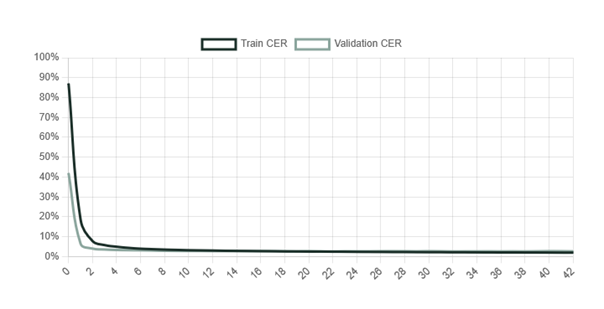
\includegraphics[width=0.7\textwidth]{Imagens/fig-000.png} 
\caption{Curva de aprendizado da última versão do EPP.}
\label{fig:curva_aprendizado}
\source{Reprodução de metadados do modelo, disponível em: \url{https://app.transkribus.org/models/text/267229}.}
\end{figure}

A análise da curva de aprendizado da versão final do modelo EPP (\Cref{fig:curva_aprendizado}) demonstra um processo de treinamento bem-sucedido. Ainda nas primeiras épocas de treinamento, há uma fase de convergência rápida, na qual o \textit{Train CER }cai de aproximadamente 85\% e o \textit{Validation CER} de aproximadamente 45\% para um patamar inferior a 10\% já nas primeiras épocas. A queda acentuada em ambas as curvas descarta um caso de underfitting. Mais importante, a distância mínima e estável entre as duas linhas demonstra que o modelo generaliza bem para dados não vistos, sinal de que também não há \textit{overfitting}. Após a décima época, as curvas atingem um “platô” de convergência, se estabilizando num CER final de 2,58\% para validação e 1,91\% para treinamento. Mesmo que esses valores não atinjam o \textit{benchmark} de 0,5\% para modelos de PTR, eles representam um resultado excelente para um modelo generalista treinado num corpus diacrônico, de natureza gráfica desuniforme. A capacidade de manter um CER tão baixo num corpus que abrange a vasta diversidade tipográfica e ortográfica de três séculos (16 a 19) comprova a robustez e a alta capacidade de generalização dos modelos \textit{PyLaia} treináveis no \textit{Transkribus}.

\section{O Early Portuguese Printing}
O modelo de reconhecimento \textit{Early Portuguese Printing} foi criado em abril de 2023 para auxiliar na transcrição das obras analisadas na dissertação “O Português das ‘Obras Proueitosas’ e dos ‘Ilustres \& Muito Reuerendos Senhores’: uma análise da mudança nos padrões de colocação pronominal clítica em gramáticas portuguesas do século 15 ao 19”. O EPP teve diversas versões ao longo do seu processo de treinamento. A primeira a ser tornada pública foi a versão V-e (model ID 191805), em outubro de 2024, com 122.337 palavras treinadas e CER de 2,67\%; a segunda versão (e final até o momento) é a VI-b, com 142.606 palavras e CER de 2,58\%, publicada em janeiro de 2025.

O treinamento do modelo EPP, como dito, partiu da constatação de que faltavam opções especializadas na biblioteca pública do \textit{Transkribus} para o tipo de obra impressa necessária na pesquisa. Para fins de documentação, os modelos voltados para a língua portuguesa disponíveis na plataforma até então eram apenas os disponíveis na \Cref{tab1}.

\begin{table}[h]
\centering
\caption{Modelos de ATR do Transkribus para a língua portuguesa até julho de 2023.}
\label{tab1}
\footnotesize
\setlength{\tabcolsep}{3pt} 

\begin{tabularx}{\textwidth}{@{} >{\raggedright\arraybackslash}p{1cm} >{\raggedright\arraybackslash}X c >{\raggedright\arraybackslash}p{3.5cm} c c c @{}}
\toprule
Hand\-written/\newline{}Print & Name e ID & Centuries & {Author} & Publication & Word count & {CER} \\ \midrule

HTR & \textit{General Portuguese} M1 (35459) & 0-21 & by \href{mailto:luciafws@icloud.com}{luciafws@icloud.com} & Sep. 27, 2022 & 64.847 & 3,80\% \\ \midrule

HTR & \textit{Transkribus portuguese handwriting} M2 (45090) & -- & by Transkribus Community & Oct. 4, 2022 & 707.803 & 8,00\% \\ \midrule

PTR & \textit{Latin Portuguese Print 17th century} (41932) & 17 & by Hervé Baudry (\href{mailto:hbaudry@fcsh.unl.pt}{hbaudry@fcsh.unl.pt}) & Nov. 9, 2022 & 23.363 & 1,5\% \\ \midrule

PTR & \textit{SPJCL 17C 4.2} (52754) & -- & by \href{mailto:oliver2@sampabym.com}{oliver2@sampabym.com} & Jan. 13, 2023 & 64.324 & 1,60\% \\ \midrule

HTR &\textit{ Portuguese Handwriting 16th-19th c}. (53270) & 16-19 & by TraPrInq Project & Jul. 5, 2023 & 1.158.586 & 5,20\% \\ \midrule

PTR & \textit{ XXth century Typewritten Portuguese }(56026) & 20 & by Natalia C. Salvador & Nov. 24, 2023 & 7.468 & 2,60\% \\ 
\bottomrule
\end{tabularx}
\source{Elaborado pelo autor a partir dos dados disponíveis em \url{https://transkribus.org}.}
\end{table}

Como se pode perceber pela \Cref{tab1}, os modelos com maior treinamento em língua portuguesa eram os modelos voltados à transcrição de manuscritos. Os únicos modelos voltados à escrita impressa entre os séculos 16-19 (natureza das obras) são os modelos \textit{SPJCL 17C 4.2} (ID: 52754), da Spanish \& Portuguese Jews’ Congregation of London, que mistura o treinamento com textos em espanhol e em hebraico romanizado, o que torna a capacidade de transcrição em língua portuguesa muito difícil, e o \textit{XXth century Typewritten Portuguese}, treinado em textos já muito mais modernos. O corpus utilizado para o treinamento do EPP possui diversas características únicas que tornavam impreciso o uso de outros modelos – por se tratarem de gramáticas e obras de cunho linguístico impressas em massa desde 1536 até 1894, diversos aspectos filológicos, tipográficos e linguísticos precisavam ser levados em consideração para a construção de um modelo suficientemente eficiente em obras de diferentes momentos históricos e tecnológicos.

As obras metalinguísticas, livros como gramáticas e tratados ortográficos, utilizadas até então para a construção do modelo final são as descritas na \Cref{tab2}.

\begin{table}[h]
\centering
\caption{Corpus de gramáticas utilizado para o treinamento do EPP.}
\label{tab2}
\small
\begin{tabularx}{\textwidth}{X l c r}
\toprule
{Título} & Autor & Publ. & N. de palavras \\
\midrule
\textit{Grammatica da lingoagem portuguesa }& Fernão de Oliveira (c. 1507-1581) & 1536 & 22.974 \\
\textit{Grammatica da lingua portuguesa} & João de Barros (1496-1570) & 1540 & 23.873 \\
\textit{Origem da Lingoa portuguesa }& Duarte Nunes de Leão (c. 1530-1608) & 1606 & 21.263 \\
\textit{Orthographia da Lingua Portugueza} & Luís Caetano de Lima, C.R. (1671-1757) & 1736 & 26.997 \\
\textit{Grammatica philosophica e orthographia racional da lingua portuguesa }& Bernardo de Lima e Melo Bacellar (1736-) & 1783 & 25.219 \\
\textit{Grammatica nacional} & Francisco Júlio Caldas Aulete (1823-1878) & 1864 & 21.353 \\

\multicolumn{4}{r}{Total: 141.679\footnotemark} \\
\bottomrule
\source{\textcite{pachecorocha2025portugues}.}
\end{tabularx}
\end{table}
\footnotetext{A diferença de 927 palavras para o total do modelo EPP se deve a obras que foram parcialmente transcritas e utilizadas no treinamento do modelo ainda no início do processo, em 2023, e que não foram incluídas no corpus da dissertação.}

Guiado pelos preceitos teóricos do aprendizado de máquina para redes neurais, o modelo EPP final foi o resultado de um processo de treinamento “iterativo” conduzido ao longo de cerca de um ano, e não de um único evento de treinamento, partindo das obras mais antigas (séc. 16) às mais recentes (séc. 19). Essa forma pouco intuitiva de aprendizado “anti-curricular” \cite[p.~103]{bengio2009learning} foi a estratégia de treinamento de IA adotada sob a premissa de que, ao investir tempo e esforço iniciais na disponibilização de GTs de melhor qualidade logo no início, o modelo desenvolveria uma base de reconhecimento mais sólida e aprenderia as exceções descartáveis, formas arcaicas que não encontraria no restante do corpus. Isso ocorreria ao aprender primeiro a vasta variabilidade dos impressos antigos, para, então, refinar esse conhecimento com textos mais padronizados. A metodologia consistiu em ciclos sequenciais de treinamento, nos quais novos documentos eram progressivamente transcritos e adicionados ao conjunto de dados para treinamento de novas versões do modelo, a partir das antigas e de mais GTs. A cada ciclo, uma nova e mais robusta versão do modelo era gerada a partir da versão anterior, por meio do transfer learning já descrito. Essa abordagem permitiu que a precisão do modelo evoluísse gradualmente e o trabalho de transcrição de GTs fosse distribuído, já que se tratava de apenas um pesquisador. O treinamento das primeiras versões do modelo começou com as obras de \textcite{barros1540grammatica} e \textcite{oliveira1536grammatica}, que já contam com versões transcritas disponíveis, especialmente as edições de \textcite{barros1540grammatica} por \textcite{machado1957joaodebarros} e as de \textcite{oliveira1536grammatica} por \textcite{buescu1975gramatica}.

A etapa de transcrição para a geração das GT foi realizada diretamente na interface de edição do \textit{Transkribus eXpert client} e, alternativamente, no webapp. Para o treinamento do modelo, a transcrição buscou ser conservadora, ou seja, caracterizou-se pela ausência de modernização ortográfica ou sintática, buscando a máxima fidelidade à materialidade do texto. No ambiente digital, essa postura diplomática consiste em, basicamente, manter os caracteres encontrados nos documentos originais por meio de seus correspondentes no padrão \textit{Unicode}. Esse processo, no entanto, buscou também equilibrar a fidelidade ao corpus com a necessidade de estruturação dos dados para o treinamento do modelo, o que potencializaria a capacidade de transcrever mais obras; esse equilíbrio implica uma série de decisões que buscam tornar o treinamento mais eficiente em detrimento ao conservadorismo da transcrição. Essa seção se dedicará a explicitar esse equilíbrio e descrever as potencialidades do modelo.

No que tange à segmentação de palavras, optou-se por uma intervenção padronizada: vocábulos que aparecem unidos no original foram separados segundo a norma ortográfica atual. Inversamente, nos casos em que erros de impressão separaram graficamente uma única palavra, o espaçamento anômalo foi mantido. Tal decisão visou preservar a previsibilidade do texto para o modelo de transcrição, evitando introduzir correções que não estivessem presentes no fac-símile. Seguindo a mesma lógica, as quebras de linha, hífens e outras marcações que indicam a interrupção de uma palavra para sua continuação na linha subsequente foram igualmente preservadas na transcrição final.

\subsection{Descrição filológica do modelo}

Ao apresentar a descrição filológica do modelo EPP, essa seção buscará detalhar as decisões tomadas ao longo do processo, de forma a exemplificar o tipo de trabalho necessário para o treinamento de modelos do tipo. Cada escolha filológica não apenas interfere diretamente na fidelidade do resultado final, mas também na fidelidade e capacidade de transcrição dos resultados futuros, pois o modelo é treinado com o próprio corpus que busca transcrever, nesse caso. A natureza diacrônica do corpus, nesse ínterim, é parte desse desafio, pois as soluções dadas a problemas de transcrição dos séculos anteriores devem ser compatíveis com as tradições gráficas dos séculos posteriores. Dessa forma, portanto, nesse trecho, será exposta uma série de exemplos de decisões e formas adotadas para a transcrição e treinamento do EPP.

Em relação aos algarismos, se optou pela manutenção das formas numéricas tal como se encontram no documento de base, tanto no caso dos algarismos arábicos quanto das formas românicas, se observando, por exemplo, o uso do “I” inicial como “i” com pingo e a representação do último “i” como “j”, conforme ilustrado na \Cref{tab3}.


\begin{table}[htbp]
\centering
\caption{Exemplos de algarismos.}
\label{tab3}
\begin{tabular}{cc}
\toprule
%\begin{figure}
%\centering

\includegraphics[width=0.4\linewidth]{Imagens/fig-001.png}
%\caption{\textbf{¶ Capitolo xviij.}}
%\label{fig:grid_1}
%\end{figure} & 
%\begin{figure}
%\centering
&
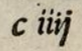
\includegraphics[width=0.1\linewidth]{Imagens/fig-002.png}
%\caption{\textbf{ciiij}}
%\label{fig:grid_2}
%\end{figure} 
\\
\textbf{¶ Capitolo xviij.} & \textbf{ciiij} \\
\bottomrule
\end{tabular}
\source{\textcite{oliveira1536grammatica,lea1606origem}, adaptado por \textcite{pachecorocha2025portugues}.}
\end{table}


O mesmo princípio de preservação foi aplicado às abreviaturas, cuja forma original foi integralmente mantida. Nesse sentido, decidiu-se unificar a representação da sobrescrição horizontal indicativa de abreviatura por meio do til ( ``\~{}''), por compreender que esta seria a intenção dos autores das obras transcritas; como demonstram os primeiros exemplos da \Cref{tab4}, o tipo-móvel utilizado para representar o (``\~{}'') parecia ser um “r” pequeno na horizontal. Além disso, se respeitou o posicionamento original do til, fosse ele colocado sobre vogais ou sobre consoantes, preservando assim as convenções gráficas observadas nos exemplares de referência, conforme demonstrado nos exemplos da \Cref{tab4}.

\begin{table}[htbp]
\centering
\caption{Exemplos de abreviaturas.}
\label{tab4}
\begin{tabular}{cccccc}
\toprule
Forma original &
\begin{subfigure}[b]{0.10\textwidth}
        \centering
        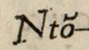
\includegraphics[width=\linewidth]{Imagens/fig-003.png}
    \end{subfigure} & 
\begin{subfigure}[b]{0.10\textwidth}
        \centering
        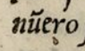
\includegraphics[width=\linewidth]{Imagens/fig-004.png}
    \end{subfigure} &
    \begin{subfigure}[b]{0.10\textwidth}
        \centering
        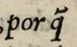
\includegraphics[width=\linewidth]{Imagens/fig-005.png}
    \end{subfigure} &
    \begin{subfigure}[b]{0.10\textwidth}
        \centering
        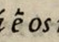
\includegraphics[width=\linewidth]{Imagens/fig-006.png}
    \end{subfigure} &
    \begin{subfigure}[b]{0.10\textwidth}
        \centering
        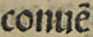
\includegraphics[width=\linewidth]{Imagens/fig-007.png}
    \end{subfigure} \\
    Transcrição adotada & \textbf{Ntõ} & \textbf{nũero} & \textbf{por q̃} & \textbf{ẽ os} & \textbf{conuẽ} \\
    Legenda & (Nominativo) & (número) & (por que) & (em os) & (convem)\footnotemark \\
    Forma original &
    \begin{subfigure}[b]{0.10\textwidth}
        \centering
        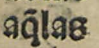
\includegraphics[width=\linewidth]{Imagens/fig-008.png}
    \end{subfigure} & 
\begin{subfigure}[b]{0.10\textwidth}
        \centering
        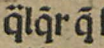
\includegraphics[width=\linewidth]{Imagens/fig-009.png}
    \end{subfigure} &
    \begin{subfigure}[b]{0.10\textwidth}
        \centering
        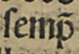
\includegraphics[width=\linewidth]{Imagens/fig-010.png}
    \end{subfigure} &
    \begin{subfigure}[b]{0.07\textwidth}
        \centering
        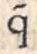
\includegraphics[width=\linewidth]{Imagens/fig-011.png}
    \end{subfigure} &
    \begin{subfigure}[b]{0.10\textwidth}
        \centering
        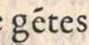
\includegraphics[width=\linewidth]{Imagens/fig-012.png}
    \end{subfigure} \\
    Transcrição adotada & \textbf{aq̃las} & \textbf{q̃lq̃r} \textbf{q̃} & \textbf{semp̃} & \textbf{q̃} & \textbf{gẽtes} \\
Legenda & (aquelas) & (qualquer que) & (sempre) & (que) & (gentes) \\
\bottomrule
\end{tabular}
\source{\textcite{oliveira1536grammatica,barros1539grammatica,lea1606origem}, adaptado por \textcite{pachecorocha2025portugues}.}
\end{table}
\footnotetext{Fernão de Oliveira não diferenciava singular e plural utilizando acentos gráficos como a convenção ortográfica moderna exige, portanto, a legenda acentuada para oxítona terminada em -em “convém”implicaria um sujeito singular (em oposição ao plural “convêm”), sentido que inexiste no documento original.}

%Inserir esta legenda que coloquei no comentário. A nota deve aparecer depois de "(convem)"


Opções como essas apresentam certos desafios, já que o número de exemplos para o treinamento precisa ser suficiente para as redes neurais aprenderem a generalizar esse tipo de ocorrência. Além disso, outros modelos do \textit{Transkribus}, baseados noutras línguas e sistemas grafemáticos, podem influenciar ou causar vícios ao modelo treinado (normalmente a “criação” de um modelo se dá a partir da especialização de outro mais próximo); modelos treinados em castelhano, por exemplo, podem generalizar formas como “ão” em “ano”. Para tal, portanto, é importante que todos os exemplos do tipo sejam devidamente transcritos e que, nas ground truths, os diacríticos estejam devidamente unidos às letras que sobrescrevem.

Em complemento a essas escolhas que buscam otimizar o trabalho de treinamento do modelo, se optou por não registrar as formas de apontamento de abreviatura cuja recorrência é reduzida diacronicamente e cuja clareza gráfica é baixa, pois a baixa nitidez de tais sinais poderia ser interpretada pelo modelo de transcrição como ruído, comprometendo o processo de treinamento. Considerou-se, nesse caso, que o eventual ganho de fidelidade filológica não se justificaria, uma vez que tais elementos são isolados e pouco numerosos o bastante para serem desconsiderados. Entre os exemplos de sinais desconsiderados, estão o uso do “r” rotundo (“{\medievalfont ꝛ}”), empregado por \textcite{oliveira1536grammatica} em todos os dígrafos com consoante complexa de tepe, como no primeiro exemplo, bem como as formas diferenciadas de abreviatura para a preposição “para” ou “pr”, observadas nos exemplos a seguir e em outras ocorrências análogas (\Cref{tab5}).

\begin{table}[htbp]
\centering
\caption{Exemplos de formas diferenciadas de abreviatura.}
\label{tab5}
\begin{tabular}{cccccc}
\toprule
Ponto de código & U+A75B & U+A751 & U+A753 & U+0223 & U+0223 \\
Forma original &
\begin{subfigure}[b]{0.17\textwidth}
        \centering
        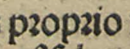
\includegraphics[width=\linewidth]{Imagens/fig-013.png}
    \end{subfigure} & 
\begin{subfigure}[b]{0.07\textwidth}
        \centering
        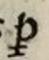
\includegraphics[width=\linewidth]{Imagens/fig-014.png}
    \end{subfigure} &
    \begin{subfigure}[b]{0.07\textwidth}
        \centering
        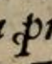
\includegraphics[width=\linewidth]{Imagens/fig-015.png}
    \end{subfigure} &
    \begin{subfigure}[b]{0.06\textwidth}
        \centering
        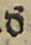
\includegraphics[width=\linewidth]{Imagens/fig-016.png}
    \end{subfigure} &
    \begin{subfigure}[b]{0.10\textwidth}
        \centering
        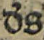
\includegraphics[width=\linewidth]{Imagens/fig-017.png}
    \end{subfigure} \\
    Transcrição adotada & \textbf{proprio} & \textbf{p} & \textbf{p} & \textbf{d} & \textbf{ds} \\
    Transcrição diplomática & {\medievalfont pꝛopꝛio} & {\medievalfont ꝑ} & {\medievalfont ꝓ} & {\medievalfont Ȣ}\footnotemark & {\medievalfont Ȣs} \\
\bottomrule
\end{tabular}
\source{\textcite{oliveira1536grammatica,barros1540grammatica}, adaptado por \textcite{pachecorocha2025portugues}.}
\end{table}
\footnotetext{Embora a transcrição adotada normalize a abreviatura para “d’”, adoto neste trabalho a hipótese de que o glifo original seja “{\medievalfont Ȣ}” (ligatura de “ou”, U+0223), provável reaproveitamento de tipos móveis destinados à impressão do grego. O uso como uma abreviação logográfica de palavras iniciadas com “d” é corroborado pela clássica transcrição de \textcite[p.~38; p.~65]{buescu1975gramatica}, que transcreve a forma “{\medievalfont Ȣs}” como “Deus”.}

%A nota de rodapé sumiu de novo

Seguindo o mesmo princípio de fidelidade, todos os diacríticos, como o acento agudo (“\'{}”), o grave (“\`{}”), o circunflexo (“\^{}”) e o til (“\~{}”), foram preservados em suas posições originais. Essa manutenção é importante, pois tais marcas refletem as convenções ortográficas do corpus e possuem função distintiva na fonética e morfologia das palavras, que não pode ser perdida. Além disso, omiti-las poderia levar o modelo de transcrição a generalizar incorretamente a exclusão de outros sinais gráficos importantes. Um caso específico de preservação foi o do e-caudata (“ę”), também chamado de “e-cedilha”, utilizado por \textcite{barros1540grammatica}. Este caractere, nomeado no padrão \textit{Unicode} como “Latin Small Letter E with Ogonek\footnote{Se trata de um glifo (Latin Small Letter E with Ogonek) atualmente utilizado na escrita de línguas como o polonês e o lituano. A adoção deste code point (U+0119) para representar o e-caudata segue as recomendações técnicas da Medieval Unicode Font Initiative \cite{haugen2015mufi}.}”, apresenta um diacrítico subscrito em forma de gancho. Sua inclusão no treinamento foi considerada essencial, pois, devido à sua proeminência visual e posicionamento em relação à letra, ignorá-lo criaria o risco de ensinar o modelo a descartar outros diacríticos subscritos, especialmente no que diz respeito à semelhança gráfica entre “c”, “e”, “ç” e “ę”, o que teria um resultado prejudicial para a precisão de qualquer transcrição em língua portuguesa (\Cref{tab6}).

\begin{table}[htbp]
\centering
\caption{Exemplos de diacrítico subscrito.}
\label{tab6}
\begin{tabular}{ccc}
\toprule
Ponto de código & U+0119 & U+0119  \\
Forma original &
\begin{subfigure}[b]{0.07\textwidth}
        \centering
        
\includegraphics[width=\linewidth]{Imagens/fig-018.png}
    \end{subfigure} & 
\begin{subfigure}[b]{0.17\textwidth}
        \centering
        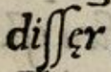
\includegraphics[width=\linewidth]{Imagens/fig-019.png}
    \end{subfigure} \\
    Transcrição adotada & \textbf{ę} & \textbf{dissęr} \\
\bottomrule
\end{tabular}
\source{\textcite{barros1540grammatica}, adaptado por \textcite{pachecorocha2025portugues}.}
\end{table}

Quanto à pontuação, todos os sinais foram preservados conforme aparecem no documento original, incluindo ponto (“.”), vírgula (“,{}”), ponto e vírgula (“;”), dois-pontos (“:”), barra (“/”), barra vertical (“|”), ponto de interrogação (“?”), ponto de exclamação (“!”), hífen (“-“), sinal de negação (“¬”) e apóstrofo (“‘”). Essa preservação buscou assegurar a fidelidade tipográfica e a interpretação correta das estruturas sintáticas, uma vez que a pontuação nos impressos históricos frequentemente apresenta variações que podem impactar a análise linguística. Além disso, se manteve a diferenciação funcional entre “u” e “v”’, herança latina ainda observada pelos autores das obras transcritas. Essa distinção, importante para a representação gráfica e fonética das palavras, foi respeitada em todos os casos do corpus, conforme ilustrado nos exemplos a seguir. No entanto, a sutileza dessa distinção pode representar um desafio para o modelo computacional. Permanece incerto se a capacidade estatística do \textit{Transkribus} é suficiente para generalizar corretamente o uso de “u” e “v” sem produzir erros, uma limitação que talvez pudesse ser superada com um volume de dados de treinamento maior ou maior dispêndio de processamento estatístico das transcrições, como o uso de modelos de linguagem ou o serviço de smart search, oferecido para os usuários pagantes (\Cref{tab7}).

\begin{table}[htbp]
\centering
\caption{Exemplos de distinção funcional “u”/”v”.}
\label{tab7}
\begin{tabular}{ccccc}
\toprule
Forma original &
\begin{subfigure}[b]{0.18\textwidth}
        \centering
        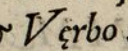
\includegraphics[width=\linewidth]{Imagens/fig-020.png}
    \end{subfigure} & 
\begin{subfigure}[b]{0.14\textwidth}
        \centering
        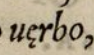
\includegraphics[width=\linewidth]{Imagens/fig-021.png}
    \end{subfigure} &
    \begin{subfigure}[b]{0.17\textwidth}
        \centering
        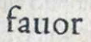
\includegraphics[width=\linewidth]{Imagens/fig-022.png}
    \end{subfigure} & 
    \begin{subfigure}[b]{0.17\textwidth}
        \centering
        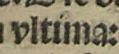
\includegraphics[width=\linewidth]{Imagens/fig-023.png}
    \end{subfigure} \\
    Transcrição adotada & \textbf{Vęrbo} & \textbf{uęrbo} & \textbf{fauor} & \textbf{vltima:}  \\
\bottomrule
\end{tabular}
\source{\textcite{oliveira1536grammatica,barros1540grammatica,lea1606origem}, adaptado por \textcite{pachecorocha2025portugues}.}
\end{table}

O tratamento das ligaturas (elementos tipográficos que unem dois ou mais caracteres em um único tipo) também exigiu a definição de um critério claro. Nas gramáticas transcritas, as ligaturas aparecem em duas formas básicas: a consonantal, que cumpria uma função pragmática de facilitar o trabalho do tipógrafo (por exemplo, criando um tipo único “{\medievalfont st}” para a sequência “st”, que exigiria dois tipos); e a vocálica, cujo uso aparenta ter também uma motivação ortográfica, especialmente em passagens em latim. Contudo, a prática de transcrição revelou que o emprego de ambas as formas é bastante idiossincrático e pouco coerente ao longo do corpus. Diante dessa inconsistência e de desafios técnicos adicionais, a norma adotada foi, via de regra, ignorar as ligaturas, desfazendo-as em seus caracteres componentes. Esta decisão foi fundamentada por três fatores principais: primeiro, a baixa representatividade da maioria das ligaturas não justificava o complexo esforço de treinamento; segundo, o risco de que formas raras fossem confundidas com ruídos do fac-símile pelo modelo, comprometendo a transcrição; e, por fim, a inexistência de certas ligaturas no padrão Unicode, o que impedia a correta representação digital das ligaturas por completo (\Cref{tab8}).

\begin{table}[htbp]
\centering
\caption{Exemplos de ligaturas tipográficas.}
\label{tab8}
\begin{tabular}{p{3cm} p{3cm} p{3cm} p{3cm}}
\toprule
Ponto de código & U+FB06 & U+FB05 & -- \\
Glifo original &
\begin{subfigure}[b]{0.18\textwidth}
        \centering
        
\includegraphics[width=\linewidth]{Imagens/fig-024.png}
    \end{subfigure} & 
\begin{subfigure}[b]{0.14\textwidth}
        \centering
        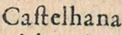
\includegraphics[width=\linewidth]{Imagens/fig-025.png}
    \end{subfigure} &
    \begin{subfigure}[b]{0.17\textwidth}
        \centering
        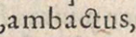
\includegraphics[width=\linewidth]{Imagens/fig-026.png}
    \end{subfigure} \\
    Transcrição adotada & \textbf{Aristoteles} & \textbf{Castelhana} & \textbf{ambactus} \\
    Transcrição diplomática & {\medievalfont Aristoteles} & {\medievalfont Caſtelhana} & Sem correspondência da ligatura no Unicode \\
\bottomrule
\end{tabular}
\source{\textcite{barros1540grammatica,lea1606origem}, adaptado por \textcite{pachecorocha2025portugues}.}
\end{table}

À norma geral de desfazer as ligaturas foi estabelecida uma única exceção: as formadas pela combinação das variantes da letra “s”. Nos textos, se observam tanto a forma “s-longo” (“{\medievalfont ſ}”) quanto a “s-curta” (“s”), cuja distinção era meramente funcional, pouco sistemática e foi, via de regra, ignorada para transcrição e treinamento. A junção das duas, no entanto, formava um caractere específico, a ligatura conhecida atualmente como eszett (“{\medievalfont ß}”). A decisão de preservar esse caractere se fundamenta basicamente na sua saliência gráfica, que é proeminente o suficiente para comprometer o treinamento do modelo caso fosse ignorada. Portanto, para garantir a estabilidade e a precisão do reconhecimento, esta ligatura em particular foi mantida na transcrição final (\Cref{tab9}).

\begin{table}[htbp]
\centering
\caption{Exemplos de distinção “s-curto”/”s-longo” e sua ligatura.}
\label{tab9}
\begin{tabular}{ccccc}
\toprule
Ponto de código & U+017F & U+00DF & U+00DF & U+0073  \\
Forma original &
\begin{subfigure}[b]{0.10\textwidth}
        \centering
        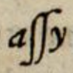
\includegraphics[width=\linewidth]{Imagens/fig-027.png}
    \end{subfigure} & 
\begin{subfigure}[b]{0.13\textwidth}
        \centering
        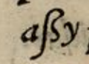
\includegraphics[width=\linewidth]{Imagens/fig-028.png}
    \end{subfigure} &
    \begin{subfigure}[b]{0.20\textwidth}
        \centering
        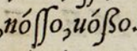
\includegraphics[width=\linewidth]{Imagens/fig-029.png}
    \end{subfigure} &
    \begin{subfigure}[b]{0.13\textwidth}
        \centering
        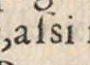
\includegraphics[width=\linewidth]{Imagens/fig-030.png}
    \end{subfigure} \\
    Transcrição adotada & \textbf{assy} & \textbf{aßy} &\textbf{ nósso,uóßo.} & \textbf{,assi}  \\
    Transcrição diplomática & {\medievalfont aſſy} & {\medievalfont aßy} & {\medievalfont nóſſo,uóßo.} & {\medievalfont ,aſsi} \\
\bottomrule
\end{tabular}
\source{\textcite{barros1540grammatica,lea1606origem}, adaptado por \textcite{pachecorocha2025portugues}.}
\end{table}

O tratamento de outros casos específicos incluiu a manutenção de nexos vocálicos, como a ligatura “{\medievalfont æ}”. De modo semelhante, se optou por preservar o “e comercial” (“\&”), a forma ligada da conjunção latina “et”, de modo a uniformizar a representação da conjunção coordenativa numa única forma sempre que esta aparecia como uma ligatura ou na notação tironiana adotada por \textcite{oliveira1536grammatica} (\Cref{tab10}).

\begin{table}[htbp]
\centering
\caption{Exemplos de outras ligaturas.}
\label{tab10}
\begin{tabular}{cccccc}
\toprule
Ponto de código & U+00C6 & U+00E6 & U+0026 & U+0026 & U+204A \\
Forma original &
\begin{subfigure}[b]{0.12\textwidth}
        \centering
        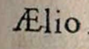
\includegraphics[width=\linewidth]{Imagens/fig-031.png}
    \end{subfigure} & 
\begin{subfigure}[b]{0.14\textwidth}
        \centering
        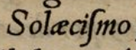
\includegraphics[width=\linewidth]{Imagens/fig-032.png}
    \end{subfigure} &
    \begin{subfigure}[b]{0.09\textwidth}
        \centering
        
\includegraphics[width=\linewidth]{Imagens/fig-033.png}
    \end{subfigure} &
    \begin{subfigure}[b]{0.08\textwidth}
        \centering
        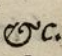
\includegraphics[width=\linewidth]{Imagens/fig-034.png}
    \end{subfigure} &
    \begin{subfigure}[b]{0.06\textwidth}
        \centering
        
\includegraphics[width=\linewidth]{Imagens/fig-035.png}
    \end{subfigure} \\
    Transcrição adotada & \textbf{{\medievalfont Ælio}} & \textbf{{\medievalfont Solæcismo}} & \textbf{\&} & \textbf{\&c} & \textbf{\&} \\
    Transcrição diplomática & {\medievalfont Ælio} & {\medievalfont Solæcismo} & \& & \&c & {\medievalfont ⁊} \\
\bottomrule
\end{tabular}
\source{\textcite{oliveira1536grammatica,barros1540grammatica,lea1606origem}, adaptado por \textcite{pachecorocha2025portugues}.}
\end{table}

O tratamento de caracteres não latinos e formas tipográficas especiais também seguiu critérios específicos. Um caso notável é a presença de letras do alfabeto grego. Devido à forte ligação do conhecimento letrado da época com a cultura greco-latina, a ocorrência desses caracteres é relativamente frequente nas gramáticas transcritas. Diante de sua relevância contextual, se optou por manter todas as letras gregas na transcrição, garantindo assim a máxima fidelidade ao texto original (\Cref{tab11}).

\begin{table}[htbp]
\centering
\caption{Exemplos de caracteres gregos.}
\label{tab11}
\begin{tabular}{ccccc}
\toprule
Ponto de código & U+0398 & U+03A6 & U+03B5 & U+03C9 \\
Forma original &
\begin{subfigure}[b]{0.12\textwidth}
        \centering
        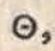
\includegraphics[width=\linewidth]{Imagens/fig-036.png}
    \end{subfigure} & 
\begin{subfigure}[b]{0.12\textwidth}
        \centering
        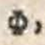
\includegraphics[width=\linewidth]{Imagens/fig-037.png}
    \end{subfigure} &
    \begin{subfigure}[b]{0.09\textwidth}
        \centering
        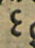
\includegraphics[width=\linewidth]{Imagens/fig-038.png}
    \end{subfigure} &
    \begin{subfigure}[b]{0.12\textwidth}
        \centering
        
\includegraphics[width=\linewidth]{Imagens/fig-039.png}
    \end{subfigure}  \\
    Transcrição adotada & Θ & Φ & \textbf{$\mathcal{E}$} & \textbf{$\omega$} \\
\bottomrule
\end{tabular}
\source{\textcite{oliveira1536grammatica,barros1540grammatica}, adaptado por \textcite{pachecorocha2025portugues}.}
\end{table}

Contudo, a essa norma de preservação aplicou-se um critério de otimização para letras gregas com formas visualmente análogas às latinas, como as maiúsculas Chi (“$\symbol{"03A7}$”, U+03A7) e Zeta (“$\symbol{"0396}$”, U+0396). Nesses casos, optou-se por transcrevê-las utilizando seus equivalentes latinos (“X”, U+0058 e “Z”, U+005A), a fim de reduzir o conjunto de caracteres a ser aprendido pelo modelo. Uma exceção crucial a este critério de simplificação foi a letra alfa latina pequena (“{\medievalfont ɑ}”, U+0251). Esse caractere, empregado por Oliveira (1536) para marcar uma distinção explícita com a letra “a” em sua proposta ortográfica, foi mantido em sua forma original, pois sua normalização tornaria o argumento do autor incompreensível. Embora a raridade do “{\notofont\char"0251}” torne seu reconhecimento pelo modelo pouco confiável, o impacto dessa decisão na performance geral do sistema foi considerado irrisório, dada sua frequência de uso extremamente baixa em comparação com a vogal “a” (\Cref{tab12}).

\begin{table}[htbp]
\centering
\caption{Exemplo de letra latina diferencial.}
\label{tab12}
\begin{tabular}{cc}
\toprule
Ponto de código & U+0251 \\
Forma original &
\begin{subfigure}[b]{0.07\textwidth}
        \centering
        
\includegraphics[width=\linewidth]{Imagens/fig-040.png}
    \end{subfigure}  \\
    Transcrição adotada & {\medievalfont ɑ} \\
\bottomrule
\end{tabular}
\source{\textcite{oliveira1536grammatica}, adaptado por \textcite{pachecorocha2025portugues}.}
\end{table}

O tratamento de elementos tipográficos e ornamentais seguiu um critério de frequência e relevância no corpus. Símbolos de presença constante, como o \textit{pilcrow} ou caldeirão (“{\medievalfont ¶}”) e os diferentes tipos de fleurão (“{\medievalfont ❧}”), foram mantidos na transcrição para preservar a estrutura visual e editorial das obras. No entanto, se optou por ignorar distinções sutis dentro de uma mesma categoria de símbolo quando a representatividade de uma das variantes era baixa. Foi o caso do caldeirão de capítulo, conhecido como \textit{capitulum} (“{\medievalfont \capitulum}”), que foi representado de forma unificada como um caldeirão simples (“{\medievalfont ¶}”), dada a sua rara ocorrência (\Cref{tab13}).

\begin{table}[htbp]
\centering
\caption{Exemplos de elementos tipográficos funcionais.}
\label{tab13}
\begin{tabular}{ccc}
\toprule
Ponto de código & U+00B6 & U+2E3F \\
Forma original &
\begin{subfigure}[b]{0.07\textwidth}
        \centering
        
\includegraphics[width=\linewidth]{Imagens/fig-041.png}
    \end{subfigure} & 
    \begin{subfigure}[b]{0.10\textwidth}
        \centering
        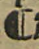
\includegraphics[width=\linewidth]{Imagens/fig-042.png}
    \end{subfigure} \\
    Transcrição adotada & {\medievalfont ¶} & {\medievalfont ¶} \\
    Transcrição diplomática & {\medievalfont ¶} & {\notofont\symbol{"2E3F}} \\
\bottomrule
\end{tabular}
\source{\textcite{oliveira1536grammatica,barros1540grammatica}, adaptado por \textcite{pachecorocha2025portugues}.}
\end{table}


Da mesma forma que o caldeirão, outros elementos ornamentais foram preservados com base em sua frequência e clareza. É o caso do fleurão, também chamado de “hera”, um elemento decorativo de uso recorrente, especialmente por \textcite{barros1540grammatica}. Sua forma graficamente distinta e seu uso frequente justificaram a decisão não apenas de mantê-lo na transcrição, mas também de incluir seu reconhecimento como uma tarefa específica no treinamento do modelo, garantindo que não fosse interpretado como ruído (\Cref{tab14}).

\begin{table}[htbp]
\centering
\caption{Exemplos de elementos tipográficos funcionais/ornamentais.}
\label{tab14}
\begin{tabular}{cccc}
\toprule
Ponto de código & U+2767 & U+2619 & U+2766 \\
Forma original &
\begin{subfigure}[b]{0.10\textwidth}
        \centering
        
\includegraphics[width=\linewidth]{Imagens/fig-043.png}
    \end{subfigure} & 
    \begin{subfigure}[b]{0.10\textwidth}
        \centering
        
\includegraphics[width=\linewidth]{Imagens/fig-044.png}
    \end{subfigure} & 
    \begin{subfigure}[b]{0.08\textwidth}
        \centering
        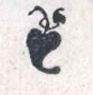
\includegraphics[width=\linewidth]{Imagens/fig-045.png}
    \end{subfigure} \\
    Transcrição adotada & {\medievalfont ❧} & {\medievalfont ☙} & {\medievalfont ❦} \\
\bottomrule
\end{tabular}
\source{\textcite{barros1540grammatica,lea1606origem}, adaptado por \textcite{pachecorocha2025portugues}.}
\end{table}


\subsection{Potencialidades e Aplicações do Modelo EPP
}

Embora o modelo EPP tenha sido treinado primariamente com obras de natureza metalinguística impressas em Portugal, suas potencialidades se estendem muito além desse gênero textual e de suas fronteiras geográficas iniciais. Na prática, a eficácia da ferramenta está circunscrita ao idioma português e à tipografia da época, independentemente do local de impressão do documento. Durante os períodos colonial e imperial, a circulação de impressos europeus e de impressão de textos em português, como jornais, decretos, alvarás, regimentos administrativos, além das próprias gramáticas, foi fundamental na formatação da ecologia linguística do Brasil, desde os centros administrativos até as zonas de fronteira em expansão no território.

Pesquisadores brasileiros que se debruçam sobre esses acervos impressos de circulação colonial podem usufruir do EPP de duas maneiras: a primeira é a aplicação direta do modelo sobre documentos impressos em língua portuguesa entre os séculos 16 e 19, a partir de sua versão disponibilizada publicamente na biblioteca do \textit{Transkribus}. Isso permite a extração automatizada de textos em larga escala e com alta confiabilidade, de maneira a viabilizar análises quantitativas que levariam anos caso dependessem de transcrição manual. A segunda, e talvez mais promissora, é o uso do EPP como um “modelo de base”. Para pesquisadores que trabalham com corpora em língua portuguesa que apresentam variações tipográficas muito específicas, não é necessário iniciar um treinamento do zero. Equipes de pesquisa podem aplicar o EPP como base e realizar o fine-tuning fornecendo apenas algumas dezenas de páginas do seu corpus específico. Essa dinâmica de transferência de aprendizado reduz drasticamente a barreira técnica e a necessidade de transcrição de corpora massivos para o treinamento a partir do zero, democratizando o alcance de um baixo CER independentemente da especificidade do material analisado.

\section{Considerações Finais}

O presente trabalho demonstrou a viabilidade e a eficácia da criação de modelos de reconhecimento de texto especializados para corpora históricos. Por meio de um processo de treinamento iterativo na plataforma \textit{Transkribus}, o modelo EPP alcançou uma Taxa de Erro de Caracteres (CER) de 2,58\% num corpus diacrônico de alta complexidade. Esse resultado comprova que a “Quarta Geração” de tecnologias de ATR, baseada em redes neurais profundas, permite que pesquisadores individuais ou pequenas equipes superem o tradicional gargalo da transcrição manual, viabilizando as análises quantitativas em larga escala exigidas pela Linguística de Corpus, que antes eram pouco concebíveis.

Contudo, a adoção de plataformas como o \textit{Transkribus}, apesar de seus inegáveis benefícios técnicos, suscita importantes questionamentos sobre a infraestrutura da pesquisa digital. É natural que a dependência de uma solução centralizada e gerida por uma entidade europeia, na qual dados e modelos que representam o patrimônio documental e científico brasileiro são processados e armazenados, tensione o debate sobre a soberania digital. Por outro lado, para que essa crítica não se encerre no mero ceticismo tecnológico, é fundamental resgatar a natureza cooperativa da READ-COOP SCE. Conforme demonstrado por \textcite[p.4~5]{terras2025artificial} e discutido ao longo deste trabalho, a plataforma é gerida sob um regime legal que foge à lógica corporativa tradicional de maximização de lucros e obriga uma gestão controlada pelos membros da cooperativa. Como não-membros da cooperativa, os usuários gratuitos do serviço não estão desprovidos de alternativas.

O desafio atual não reside na ausência de ferramentas alinhadas a uma filosofia de ciência aberta, mas sim nas condições estruturais para a sua adoção. Plataformas de código aberto e acesso livre, como o \textit{eScriptorium} (baseado no motor Kraken), já permitem o processamento de documentos em servidores institucionais próprios. Adicionalmente, também nada impede que pesquisadores operem motores como o próprio PyLaia de forma autônoma, por meio de scripts locais, dispensando interfaces comerciais. Entretanto, a adoção prática dessas alternativas esbarra numa limitação de formação tecnológica, ecossistema e usabilidade. Diferentemente do Transkribus, que atua como um agregador com biblioteca de modelos pública nativa, as soluções abertas possuem uma dinâmica fragmentária. Embora existam louváveis catálogos independentes mantidos pela comunidade, como o diretório HTR-United, eles operam de forma externa à ferramenta de transcrição. Essa necessidade de buscar, baixar arquivos em repositórios de dados (como o Zenodo) e importá-los manualmente para, assim, testar sua aplicabilidade ao corpus desejado eleva a curva de adoção técnica e dificulta o reuso de modelos pré-treinados por pesquisadores cuja especialidade não é tecnologia, mas paleografia, linguística etc. Na prática, essa fricção no compartilhamento leva equipes a iniciarem seus treinamentos a partir do zero.

Além disso, a transição para um modelo puramente descentralizado de inteligência artificial enfrenta grandes obstáculos, especialmente no contexto do financiamento da ciência pública brasileira. Primeiramente, o processamento e o treinamento de redes neurais exigem um hardware custoso, cuja aquisição e manutenção pulverizada por diferentes universidades se mostra financeiramente difícil no cenário atual. Em segundo lugar, a descentralização excessiva do processamento fragmenta os corpora; ao treinar modelos isoladamente em computadores locais, a comunidade perde a capacidade de escalonamento colaborativo. A centralização de dados é uma condição para pesquisa com IA e o treinamento de modelos generalistas, como os do \textit{Transkribus}, treinados com milhões de palavras, dependem fundamentalmente do acúmulo e da centralização de dados e de trabalho humano. Embora plataformas de código aberto como o \textit{eScriptorium permitam }o trabalho colaborativo e o compartilhamento interno de modelos entre usuários de um mesmo projeto, essa funcionalidade é restrita ao ambiente em que o sistema está hospedado. Sua implementação exige, invariavelmente, a manutenção de um servidor institucional dedicado. Sem um projeto interinstitucional que centralize os custos de processamento e o armazenamento de uma biblioteca de modelos à semelhança do modelo cooperativo europeu, a alternativa ao \textit{Transkribus} no Brasil seria esperar que os pesquisadores brasileiros tenham o conhecimento técnico necessário e poder de processamento em suas máquinas pessoais, cenário que ainda inviabilizaria a organização do trabalho colaborativo.

Dessa forma, a sustentabilidade e a autonomia da pesquisa nacional no treinamento de modelos de HTR para transcrição de corpora históricos exigem, mais do que a mera adoção de tecnologias livres, a consolidação de uma estrutura de pesquisa capaz de planificar investimentos em infraestrutura tecnológica e em bases de dados integradas. Mediante uma organização do tipo, seria possível desenvolver alternativas reais, públicas e nacionais ao modelo da sociedade cooperativa europeia. Em suma, a despeito das críticas legítimas, a iniciativa europeia conseguiu alcançar, dentro de suas limitações, um ecossistema colaborativo e, de certa forma, gratuito, erigindo, nas palavras de \textcite{terras2025artificial}, uma verdadeira “infraestrutura comunitária compartilhada”.

Ainda assim, o trabalho metodológico descrito em torno do modelo EPP aponta para um futuro promissor e alinhado aos princípios da Ciência Aberta. Para superar o entrave da centralização corporativa e garantir que o modelo se consolide como uma ferramenta de acesso livre e amplo, o compromisso deste trabalho se estende à disponibilização pública de seus dados formadores. Ao tornar o corpus e os parâmetros do modelo publicamente acessíveis sob licenças abertas, garante-se a interoperabilidade dos dados. Na prática, isso permite que a comunidade acadêmica exporte esse conhecimento e o aplique diretamente em ecossistemas fundamentados em software livre, como o próprio eScriptorium, ou em instâncias locais do \textit{PyLaia}. Mais do que uma ferramenta de transcrição restrita a um único ambiente, o EPP representa um ativo de pesquisa e dados abertos que pode ser continuamente aprimorado, auditado e aplicado a novos acervos. Dessa forma, acelera-se o trabalho de filólogos, historiadores e linguistas, buscando promover a colaboratividade e garantir que o avanço das Humanidades Digitais sobre os vestígios escritos do passado seja, em sua essência, um bem comum, auditável e inalienável.

\printbibliography\label{sec-bib}
% if the text is not in Portuguese, it might be necessary to use the code below instead to print the correct ABNT abbreviations [s.n.], [s.l.]
%\begin{portuguese}
%\printbibliography[title={Bibliography}]
%\end{portuguese}



\begin{dataavailability}
\txtdataavailability{dataavailable} % options: dataavailable, dataonly, databody, datanotav, nodata
\end{dataavailability}

\begin{funding}
O presente trabalho foi realizado com apoio da Coordenação de Aperfeiçoamento de Pessoal de Nível Superior - Brasil (CAPES) - Código de Financiamento 001.
\end{funding}

\section*{\fontsize{10}{12}\selectfont Declaração de disponibilidade de dados de pesquisa}
Em conformidade com as práticas de Ciência Aberta, o \textit{dataset} de gramáticas e obras metalinguísticas utilizado para o treinamento e validação do modelo \textit{Early Portuguese Printing} (EPP) está depositado publicamente no repositório Zenodo. O conjunto de dados inclui os fac-símiles das obras em PDF com camada de texto (ATR), o banco de dados relacional em formato SQLite (.db), que integra o texto integral a metadados estratificados (autor, nascimento, publicação e título), e as transcrições em arquivos de texto plano (.txt) para máxima interoperabilidade. Os dados podem ser acessados livremente e citados por meio do identificador de objeto digital: \url{https://doi.org/10.5281/zenodo.18354169}.

\section*{\fontsize{10}{12}\selectfont Declaração de conflitos de interesses}
O autor declara que a pesquisa foi conduzida na ausência de quaisquer relações comerciais ou financeiras que possam ser interpretadas como um potencial conflito de interesses.



\end{document}

